\documentclass[journal,hidelinks]{IEEEtran}
\usepackage[utf8]{inputenc}
\usepackage[
  pdftitle={Assignment \#2},
  pdfauthor={Andrei Purcarus},
  pdfsubject={ECSE-543 -- Numerical Methods in EE}
]{hyperref}
\usepackage{graphicx}
\usepackage[all]{hypcap}
\usepackage{amsmath}
\usepackage{amssymb}
\usepackage{cleveref}
\usepackage{indentfirst}
\usepackage[per-mode=symbol]{siunitx}
\usepackage{listings}
\lstset{showstringspaces=false}

\title{ECSE-543 \\ Numerical Methods in EE \\ Assignment \#2}
\author{Andrei~Purcarus,~260631911,~\IEEEmembership{McGill~University}}

\begin{document}
\sloppy

\maketitle

\section*{Code Listings and Unit Testing}

The source code used for this assignment is listed in the appendices. In order to save space, we did not include the unit tests. For the full code, see the \href{https://github.com/Gripnook/ECSE543-F17-A2}{GitHub repository}.

\Cref{sec:q2a-py} contains the code used in Question 2 to generate the input data file for Simple2D. \Cref{sec:q2c-py} contains the code used in Question 2 to solve for the capacitance per unit length. \Cref{sec:main} contains the main function for Question 3. \Cref{sec:matrix,sec:matrix-util} define a matrix library and helper functions. \Cref{sec:cholesky} defines functions that perform Cholesky decomposition using banded and non-banded methods. \Cref{sec:solver} defines a generic solver for systems of equations that have a positive definite coefficient matrix. \Cref{sec:finite-differences-h,sec:finite-differences-cpp} define a finite difference problem generator. Finally, \Cref{sec:conjugate-gradient} defines a conjugate gradient solver for systems of equations that have a positive definite coefficient matrix.

\section*{Question 1}

We started by computing the potential for the triangle composed of nodes $(1,2,3)$. Using a linear approximation for the potential inside the triangle, we have
\begin{equation}
\label{eq:potential}
U = a + b x + c y =
\begin{bmatrix}
1 & x & y \\
\end{bmatrix}
\begin{bmatrix}
a \\
b \\
c \\
\end{bmatrix}
= \boldsymbol{x}^T \boldsymbol{\alpha}
\end{equation}

Using \Cref{eq:potential} and the potentials $U_1$, $U_2$, and $U_3$ at the nodes, we obtain
\begin{equation}
\label{eq:potential_system}
\boldsymbol{u} =
\begin{bmatrix}
U_1 \\
U_2 \\
U_3 \\
\end{bmatrix}
=
\begin{bmatrix}
1 & x_1 & y_1 \\
1 & x_2 & y_2 \\
1 & x_3 & y_3 \\
\end{bmatrix}
\begin{bmatrix}
a \\
b \\
c \\
\end{bmatrix}
=
\boldsymbol{X} \boldsymbol{\alpha} \\
\end{equation}

Using \Cref{eq:potential,eq:potential_system} together yields
\begin{equation}
U = \boldsymbol{x}^T \boldsymbol{X}^{-1} \boldsymbol{u}
\end{equation}

We next moved to finding the energy in the triangle, which is given by
\begin{align}
W &= \frac{1}{2} \int_{\Delta} |\boldsymbol{\nabla} U|^2 dS \\
  &= \frac{1}{2} \int_{\Delta} |\boldsymbol{\nabla} (\boldsymbol{x}^T \boldsymbol{X}^{-1} \boldsymbol{u})|^2 dS \\
  &= \frac{1}{2} \int_{\Delta} |\boldsymbol{Z} \boldsymbol{X}^{-1} \boldsymbol{u}|^2 dS \\
  &= \frac{1}{2} \boldsymbol{u}^T (\int_{\Delta} (\boldsymbol{Z} \boldsymbol{X}^{-1})^T \boldsymbol{Z} \boldsymbol{X}^{-1} dS) \boldsymbol{u} \\
  &= \frac{1}{2} \boldsymbol{u}^T (A (\boldsymbol{Z} \boldsymbol{X}^{-1})^T \boldsymbol{Z} \boldsymbol{X}^{-1}) \boldsymbol{u} \\
  &= \frac{1}{2} \boldsymbol{u}^T \boldsymbol{S} \boldsymbol{u}
\end{align}
where $A$ is the area of the triangle, and
\begin{equation}
\boldsymbol{Z} =
\begin{bmatrix}
0 & 1 & 0 \\
0 & 0 & 1 \\
\end{bmatrix}
\end{equation}

We then computed by hand
\begin{equation}
A_1 = \frac{1}{2} 0.02 \cdot 0.02 = \frac{1}{5000}
\end{equation}
\begin{equation}
\boldsymbol{X}^{-1}_1 =
\begin{bmatrix}
1 & 0.00 & 0.02 \\
1 & 0.00 & 0.00 \\
1 & 0.02 & 0.02 \\
\end{bmatrix}^{-1} =
\begin{bmatrix}
0 & 1 & 0\\
0 & -50 & 50 \\
-50 & 50 & 0 \\
\end{bmatrix}
\end{equation}
\begin{equation}
\boldsymbol{Z} \boldsymbol{X}^{-1}_1 =
\begin{bmatrix}
0 & -50 & 50 \\
-50 & 50 & 0 \\
\end{bmatrix}
\end{equation}
\begin{align}
\boldsymbol{S}_{dis,1} &= A_1 (\boldsymbol{Z} \boldsymbol{X}^{-1}_1)^T \boldsymbol{Z} \boldsymbol{X}^{-1}_1 \\
&= \begin{bmatrix}
0.5 & -0.5 & 0.0 \\
-0.5 & 1.0 & -0.5 \\
0.0 & -0.5 & 0.5 \\
\end{bmatrix}
\end{align}

Similarly, we computed
\begin{align}
\boldsymbol{S}_{dis,2} &= A_2 (\boldsymbol{Z} \boldsymbol{X}^{-1}_2)^T \boldsymbol{Z} \boldsymbol{X}^{-1}_2 \\
&= \begin{bmatrix}
1.0 & -0.5 & -0.5 \\
-0.5 & 0.5 & 0.0 \\
-0.5 & 0.0 & 0.5 \\
\end{bmatrix}
\end{align}

To compute the conjoint matrix $\boldsymbol{S}_{con}$, we used the fact that
\begin{align}
W &= \frac{1}{2} \boldsymbol{u}^T_{con} \boldsymbol{S}_{con} \boldsymbol{u}_{con} \\
  &= \frac{1}{2} \boldsymbol{u}^T_{dis} \boldsymbol{S}_{dis} \boldsymbol{u}_{dis}
\end{align}
where
\begin{equation}
\boldsymbol{u}_{dis} =
\begin{bmatrix}
U_1 \\
U_2 \\
U_3 \\
U_4 \\
U_5 \\
U_6 \\
\end{bmatrix} =
\begin{bmatrix}
1 & 0 & 0 & 0 \\
0 & 1 & 0 & 0 \\
0 & 0 & 1 & 0 \\
0 & 0 & 0 & 1 \\
1 & 0 & 0 & 0 \\
0 & 0 & 1 & 0 \\
\end{bmatrix}
\begin{bmatrix}
U_1 \\
U_2 \\
U_3 \\
U_4 \\
\end{bmatrix} =
\boldsymbol{C} \boldsymbol{u}_{con}
\end{equation}
and
\begin{equation}
\boldsymbol{S}_{dis} =
\begin{bmatrix}
\boldsymbol{S}_{dis,1} & 0 \\
0 & \boldsymbol{S}_{dis,2} \\
\end{bmatrix}
\end{equation}

Putting all of this together, we obtained
\begin{align}
\boldsymbol{S}_{con} &= \boldsymbol{C}^T \boldsymbol{S}_{dis} \boldsymbol{C} \\
\label{eq:s-con}
&=
\begin{bmatrix}
1.0 & -0.5 & 0.0 & -0.5 \\
-0.5 & 1.0 & -0.5 & 0.0 \\
0.0 & -0.5 & 1.0 & -0.5 \\
-0.5 & 0.0 & -0.5 & 1.0 \\
\end{bmatrix}
\end{align}

\section*{Question 2}

\subsection*{(a)}

We divided the mesh as instructed with a uniform $\SI{0.02}{\meter}$ spacing on each axis, then subdivided each resulting square with the same triangle setup as was given in Question 1.
In order to generate the finite elements mesh file for use with Simple2D, we used the program shown in \Cref{sec:q2a-py}. This program generated the file shown in \Cref{sec:file-dat}.

\subsection*{(b)}

We then used the file in \Cref{sec:file-dat} as input to the Simple2D Matlab program provided for this assignment and exported the resulting node potentials to a file, as given in \Cref{sec:results-dat}. From this file, we can see that the potential at the point (0.06, 0.04), which corresponds to node 21, is $\SI{5.5263}{\volt}$. This agrees with the value we obtained in Assignment \#1 for the same grid spacing, which was exactly the same when using the SOR method.

\subsection*{(c)}
\label{sec:q2c}

To compute the capacitance per unit length, we used the fact that the electrical energy density $w_e$ is given by
\begin{align}
w_e &= \frac{1}{2} \epsilon_o |\boldsymbol{E}|^2 \\
    &= \frac{1}{2} \epsilon_o |\boldsymbol{\nabla} V|^2
\end{align}

We could therefore compute the total energy per unit length in a finite element square as
\begin{align}
W &= \int_{\square} w_e dS \\
  &= \int_{\square} \frac{1}{2} \epsilon_o |\boldsymbol{\nabla} V|^2 dS \\
\label{eq:capacitance}
  &= \frac{1}{2} \epsilon_o \boldsymbol{v}^T \boldsymbol{S}_{con} \boldsymbol{v}
\end{align}
where $\boldsymbol{v}$ is the electric potential vector and $\boldsymbol{S}_{con}$ is as given in \Cref{eq:s-con}.

Then, after summing up all the energies per unit length between the conductors, we could obtain the capacitance per unit length from
\begin{equation}
W = \frac{1}{2} C' V^2
\end{equation}

A program that takes the results in \Cref{sec:results-dat} and computes the capacitance per unit length is shown in \Cref{sec:q2c-py}. The result of this program is
\begin{equation}
C' = \SI{52.1}{\pico\farad\per\meter}
\end{equation}

\section*{Question 3}

\subsection*{(a)}

We first re-purposed the old code we used in Assignment \#1 to produce the finite difference mesh, and modified it to produce matrices that could be used to solve for the potentials at each node as a system of linear equations. The resulting code is shown in \Cref{sec:finite-differences-h,sec:finite-differences-cpp}. Then, we tested the matrix $\boldsymbol{A}$ to ensure that it is positive definite using the Cholesky decomposition we wrote for Assignment \#1, and the code that does this is shown in \Cref{sec:main}. The resulting output is shown in \Cref{fig:positive_definite}. We can see that the matrix $\boldsymbol{A}$ by itself is not positive definite. To make it so, we left multiply each side of $\boldsymbol{A} \boldsymbol{x} = \boldsymbol{b}$ by $\boldsymbol{A}^T$, since $\boldsymbol{A}^T \boldsymbol{A}$ is symmetric and therefore is more likely to be positive definite. As \Cref{fig:positive_definite} shows, $\boldsymbol{A}^T \boldsymbol{A}$ is indeed positive definite, and we can use this modified system of equations instead.

\begin{figure}[!htb]
  \centering
  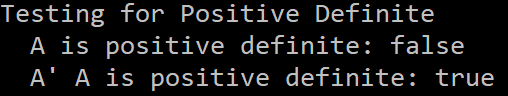
\includegraphics[width=\columnwidth]{question-3/positive_definite.png}
  \caption{The output of the program in \Cref{sec:main} for Question 3, Part (a).}
  \label{fig:positive_definite}
\end{figure}

\subsection*{(b)}

Next, we solved the system of equations given by
\begin{equation}
\boldsymbol{A}^T \boldsymbol{A} \boldsymbol{x} = \boldsymbol{A}^T \boldsymbol{b}
\end{equation}
using both Cholesky decomposition and the conjugate gradient method. The code that performs this task is shown in \Cref{sec:main}, and the code for the solvers is shown in \Cref{sec:solver,sec:conjugate-gradient}. The resulting program outputs are shown in \Cref{fig:cholesky,fig:cg}, which show the potentials in the bottom left quarter of the conductor.

\begin{figure}[!htb]
  \centering
  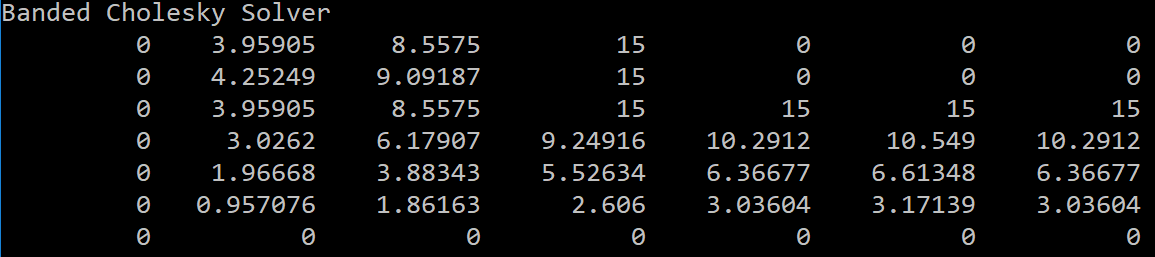
\includegraphics[width=\columnwidth]{question-3/cholesky.png}
  \caption{The output of the program in \Cref{sec:main} for the Cholesky solver in Question 3, Part (b).}
  \label{fig:cholesky}
\end{figure}

\begin{figure}[!htb]
  \centering
  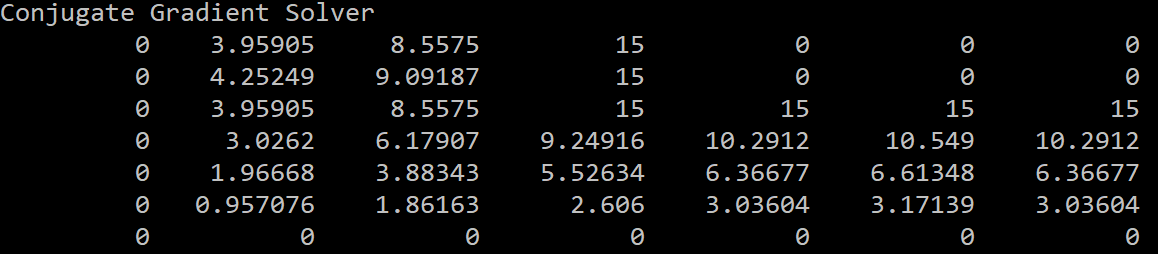
\includegraphics[width=\columnwidth]{question-3/cg.png}
  \caption{The output of the program in \Cref{sec:main} for the conjugate gradient solver in Question 3, Part (b).}
  \label{fig:cg}
\end{figure}

\subsection*{(c)}

When we executed the conjugate gradient solver, we also added a callback that computed the 2-norm and infinity norm for the residual at each iteration. The results are plotted in \Cref{fig:cg_results}. This figure shows that the conjugate gradient method does indeed reduce the residual (as given by the 2-norm) at each step, getting closer and closer to a solution. In addition, it converges to a tolerance of $10^{-5}$ in about $24$ steps for $24$ nodes, showing that it does indeed take $O(n)$ steps.

\begin{figure}[!htb]
  \centering
  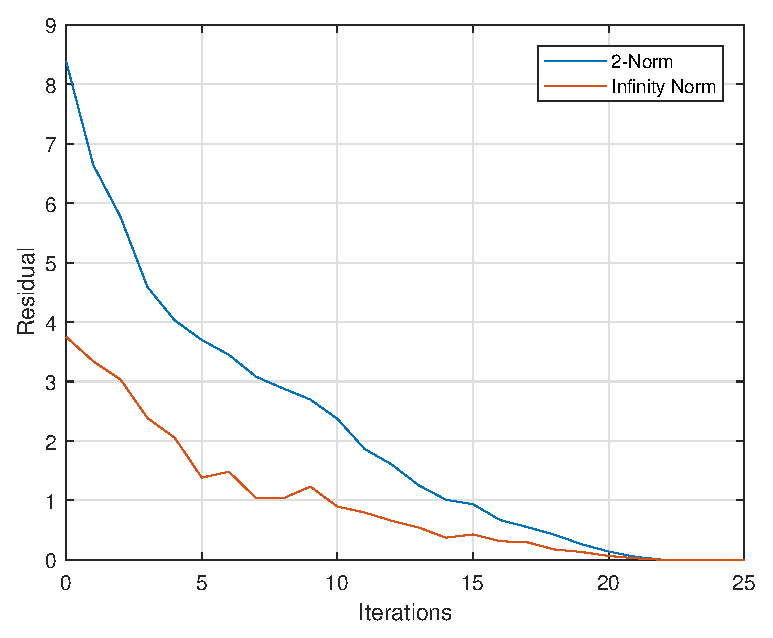
\includegraphics[width=\columnwidth]{question-3/cg_results.eps}
  \caption{2-norm and infinity norm vs. iterations for the conjugate gradient solver.}
  \label{fig:cg_results}
\end{figure}

\subsection*{(d)}

From \Cref{fig:cholesky,fig:cg}, we found that the potential at the point (0.06, 0.04) was $\SI{5.52634}{\volt}$ for both the Cholesky solver and the conjugate gradient solver. We also found a potential of $\SI{5.5263}{\volt}$ using the finite elements method, and a potential of $\SI{5.52634}{\volt}$ using the SOR method in Assignment \#1. Clearly, all of these different methods converge to the same result, which makes sense since they all use the same grid spacing and work to achieve the same tolerance of $10^{-5}$. The main difference between them is therefore the speed of convergence.

\subsection*{(e)}

To compute the capacitance per unit length using the finite difference solution obtained, we could use \Cref{eq:capacitance} to obtain the energy between the conductors, since this formula only relies on the electric potentials at the nodes in a square mesh, and hence can be used with our finite difference mesh. The rest of the calculation would be identical to the one carried out previously.

\newpage
\onecolumn

\begin{appendices}

\section{Q2a.py}
\label{sec:q2a-py}
\lstinputlisting[language=Python]{src/q2a.py}
\newpage

\section{Q2c.py}
\label{sec:q2c-py}
\lstinputlisting[language=Python]{src/q2c.py}
\newpage

\section{File.dat}
\label{sec:file-dat}
\lstinputlisting{question-2/file.dat}
\newpage

\section{Results.dat}
\label{sec:results-dat}
\lstinputlisting{question-2/results.dat}
\newpage

\section{Main.cpp}
\label{sec:main}
\lstinputlisting[language=C++]{src/main.cpp}
\newpage

\section{Matrix.h}
\label{sec:matrix}
\lstinputlisting[language=C++]{src/matrix.h}
\newpage

\section{Matrix-util.h}
\label{sec:matrix-util}
\lstinputlisting[language=C++]{src/matrix-util.h}
\newpage

\section{Cholesky.h}
\label{sec:cholesky}
\lstinputlisting[language=C++]{src/cholesky.h}
\newpage

\section{Solver.h}
\label{sec:solver}
\lstinputlisting[language=C++]{src/solver.h}
\newpage

\section{Finite-differences.h}
\label{sec:finite-differences-h}
\lstinputlisting[language=C++]{src/finite-differences.h}
\newpage

\section{Finite-differences.cpp}
\label{sec:finite-differences-cpp}
\lstinputlisting[language=C++]{src/finite-differences.cpp}
\newpage

\section{Conjugate-gradient.h}
\label{sec:conjugate-gradient}
\lstinputlisting[language=C++]{src/conjugate-gradient.h}
\newpage

\end{appendices}

\end{document}
